% !TEX root = sample.tex
%%==========================================================================
\section{SuperMatching}
\label{sec:supersymhopm}
%-------------------------------------------------------------------------
We first discuss the former two issues mentioned above, 
which are independent of application; later we turn to definition of affinity measure, which is application dependent, and sampling strategy.

\subsection{Supersymmetric affinity tensor}
\label{subsec:supersymtensor}

A tensor generalises vectors and matrices to higher dimensions: a vector is a tensor of order one,
and a matrix is a tensor of order two. A higher-order tensor can be expressed as a multi-dimensional array~\cite{Kolda08}.
Here we consider a higher-order supersymmetric affinity tensor, which represents a real-valued higher-order affinity between feature tuples.

\newtheorem{mot}{Definition}
\begin{mot}[Supersymmetric Tensor]
\label{mot:def1}
A tensor is called supersymmetric if its entries are invariant under any permutation of its indices~\cite{Kofidis02}.
\end{mot}

For example, a third-order supersymmetric tensor $\mathcal{T}_3$, satisfies the relationships:
$\mathcal{T}_3(i_1, i_2, i_3)=\mathcal{T}_3(i_1, i_3, i_2)=\mathcal{T}_3(i_2, i_1, i_3)=\mathcal{T}_3(i_2, i_3, i_1)=\mathcal{T}_3(i_3, i_1, i_2)=\mathcal{T}_3(i_3, i_2, i_1)$.

\begin{mot}[Supersymmetric Affinity Tensor]
\label{mot:def2}
Given two feature sets $P_1$ and $P_2$, with $N_1$ and $N_2$ features respectively,
the supersymmetric affinity tensor is an $N^{th}$ order $I_1\cdots \times I_N$, nonnegative tensor $\mathcal{T_N}$,
where $I_1=I_2=\cdots =I_N=\{1,\cdots,N_1N_2\}$, for which there exists a set of indices $\theta_N$,
and an $N^{th}$ order potential function $\phi_N$, such that
%
\begin{flalign}
\mathcal{T}_N(i_1,\ldots,i_N) = \begin{cases}
\phi_N(\Omega(i_1,\ldots,i_N))&{,\forall(i_1,\ldots,i_N)\in \theta_N}  \\
\quad{}\quad{}\quad{}   0     &{,\forall(i_1,\ldots,i_N)\notin \theta_N}
\end{cases}
\end{flalign}
%
where $\Omega$ stands for an arbitrary permutation of the vector, and $\theta_N$ satisfies $\forall (i_1,i_2,\ldots,i_N)\in \theta_N, \forall i_p\in\{i_1, \ldots, i_N\}$
and $\forall i_q\in\{i_1, \ldots, i_N\}-\{i_p\}$ meets the requirement that $i_p\neq i_q$.

A tensor element with $(i_1,i_2,\ldots,i_N)\in \theta_N$ is called a \emph{potential element}, while other elements are called \emph{non-potential element}.
\end{mot}

Using Definition~\ref{mot:def2}, we now can greatly reduce the amount of storage needed, representing every potential element $\mathcal{T}_N(i_1,i_2,\ldots,i_N)$ by the canonical entry $\mathcal{T}_N(\mathrm{sort}(i_1,i_2,\ldots,i_N))$, $\forall (i_1,i_2,\ldots,i_N)\in \theta_N$. Each stored value thus provides the value for $N!$ entries.
As non-potential elements all have value zero, there is no need to store them.
This greatly reduces the sampling
%%%RRM The need for sampling has still not been explained
needed for feature tuples when creating the affinity tensor, as discussed in Section~\ref{subsec:sampling}.
At the same time, it can be used to make the power iteration process more efficient: see Section~\ref{subsec:oursymmhopm}.

%-------------------------------------------------------------------------
\subsection{Higher-order Power Iteration Solving}
\label{subsec:oursymmhopm}

\begin{algorithm}[!t]
\caption{\small Higher-order power iteration method for a \protect\\
         \mbox{}\hspace{15ex}\small supersymmetric affinity tensor (with $\mathcal{C}_1$ norm)}
\label{alg2}
\begin{algorithmic}[1]
\REQUIRE \small $Nth$-order supersymmetric affinity tensor $\mathcal{T}_n$
\ENSURE  \small unit-norm vector $\boldsymbol{u}$
\STATE   \small \; Initialize $\boldsymbol{u}_0$, $k=1$
\REPEAT
    \FOR{all $(i_1,i_2,\cdots , i_N)\in \theta_N$}
        \FOR{all $m \in (i_1,\cdots , i_N)$}
        \STATE $v_{m}^{(k)}=(N-1)!\phi_N(i_1,\cdots , i_N) 2v_{m}^{(k-1)}v_{i_1}^{2_{(k-1)}}\cdots$ \\
                 $\qquad \qquad v_{m-1}^{2_{(k-1)}}v_{m+1}^{2_{(k-1)}}\cdots v_{i_N}^{2_{(k-1)}}$
        \ENDFOR
        \FOR{$i=1:N_1$}
        \STATE $v^{(k)}(((i-1)\cdot N_2+1) : i\cdot N_2)=$   \protect\\
               $\hat{v}^{(k)}(((i-1)\cdot N_2+1) : i\cdot N_2)/\lVert \hat{v}^{(k)}(((i-1)\cdot N_2+1):i\cdot N_2)\lVert_1$
        \ENDFOR
    \ENDFOR
    \STATE $k=k+1$;
\UNTIL{\small convergence};\protect\\
       \small \textbf{Note}: $v^{(k)}(((i-1)\cdot N_2+1) : i\cdot N_2)$ denotes the slice of $v^{(k)}$ with
       \small indices from $(i-1)\cdot N_2+1$ to $i\cdot N_2$.
\end{algorithmic}
\end{algorithm}

Using Definition~\ref{mot:def2}, Equ.(\ref{equ:assigment}) can be expressed as:
\begin{eqnarray}
\label{equ:assigment2}
{\boldsymbol{x}}^* &=& \argmax_{\boldsymbol{x}} \sum_{i_1,i_2,\cdots,i_N} \mathcal{T}_N(i_1,\cdots,i_N) x_{i_1},\cdots,x_{i_N} \nonumber\\
%%%RRM why are there commas after x_i1 etc?
&=& \max <\mathcal{T}_N, \boldsymbol{x}^{\star N}>
\end{eqnarray}
where $\star$ is called the Tucker product~\cite{Kofidis02}, and $\boldsymbol{x} \in \{0,1\}^{N_1N_2}$.
Solving Equ.(\ref{equ:assigment2}) is an NP-complete problem,
so it is common to relax the constraints:
the binary assignment vector $\boldsymbol{x}\in \{0,1\}^{N_1N_2}$ is replaced by an assignment vector $\boldsymbol{u}$ with elements taking real values in $[0,1]$.
This changes the optimization problem to one of computing the rank-one approximation of the affinity tensor $\mathcal{T}_N$~\cite{Kofidis02},
i.e.\ finding a scalar $\lambda$ and a unit norm vector $\boldsymbol{u}\in \mathbb{R}^{N_1N_2}$,
such that the tensor $\hat{\mathcal{T}_N} = \lambda \boldsymbol{u}\star \boldsymbol{u} \star\cdots \star \boldsymbol{u}=\boldsymbol{u}^{\star N}$ minimizes the function $f(\hat{\mathcal{T}_N})=\lVert \mathcal{T}_N-\hat{\mathcal{T}_N} \lVert$.
The final matching result is found by replacing each element of $\boldsymbol{u}$ by 0 or 1 according to whichever it is closer to.

The higher-order power method is commonly used to find the rank-one tensor approximation;
a version for supersymmetric tensors (S-HOPM) is given in~\cite{Kofidis02}.
The S-HOPM algorithm converges under the assumption of convexity for the functional induced by the tensor~\cite{Kofidis02},
which is so robust that could be satisfied in practical application.
S-HOPM is performed in two iterative steps: high-order power iteration of $\boldsymbol{u}$, normalization of $\boldsymbol{u}$ under the Frobenius norm.
In the recent, one more effective improvement~\cite{Duchenne_etal09} was proposed by using $\mathcal{C}_1$ norm to replace the traditional $\mathcal{C}_2$ norm.

We directly take the $\mathcal{C}_1$ norm~\cite{Duchenne_etal09} and further revise S-HOPM as following.
For the first step (high-order power iteration of $\boldsymbol{u}$), $\hat{\boldsymbol{u}}^{(k)}=\mathcal{I}\mathop{\star}\limits^{\mathcal{T}_N}
{(\boldsymbol{u}^{(k-1)})}^{\mathop{\star}\limits^{\mathcal{T}_N} (N-1)}$,
$\mathop{\star}\limits^{\mathcal{T}_N}$ is a so-called $\mathcal{T}_N$-product,
$\mathcal{I}$ is the unit tensor~\cite{Kofidis02}.
Then, for $\hat{\boldsymbol{u}}^{(k)}$ with $N$th-order supersymmetric affinity tensor, it can be formulated as:
\begin{flalign}
\label{equ:eqsmain2}
&\hat{\boldsymbol{u}}^{(k)}=\mathcal{I}\mathop{\star}\limits^{\mathcal{T}_N}
{(\boldsymbol{u}^{(k-1)})}^{\mathop{\star}\limits^{\mathcal{T}_N} (N-1)} \Leftrightarrow  \nonumber \\
&\forall m\in (i_1,\cdots , i_N), v_{m}^{(k)}= \nonumber\\
&\sum\limits_{i_1,\ldots,i_N}\mathcal{T}_N(i_1,\cdots,i_N)2v_{m}^{(k-1)}v_{i_1}^{2_{(k-1)}}\cdots v_{m-1}^{2_{(k-1)}}v_{m+1}^{2_{(k-1)}}\cdots v_{i_N}^{2_{(k-1)}}= \nonumber \\
&(N-1)!\phi_N(i_1,\cdots,i_N)2v_{m}^{(k-1)}v_{i_1}^{2_{(k-1)}}\cdots v_{m-1}^{2_{(k-1)}}v_{m+1}^{2_{(k-1)}}\cdots v_{i_N}^{2_{(k-1)}}
\end{flalign}
where $\boldsymbol{u}^{(k)}=\boldsymbol{v}^{2_{(k)}}$, $\phi_N$ is corresponding potential function.
The deduction relies on two principles. First, we take advantage of the supersymmetry.
Secondly, many of the elements of the affinity tensor are zero non-potential elements:
it is much more efficient to perform the power iteration by just considering the non-zero potential elements.
So, our supersymmetric higher-order power iteration solving is addressed as Algorithm~\ref{alg2}.

This version excludes each non-potential element from the iteration process, so is more efficient,
and the complexity of the whole iteration process only depends on the number $|\theta_N|$ of affinities. Step 5 in Algorithm~\ref{alg2} includes all permutations of each potential element $\mathcal{T}_n(i_1,i_2,\cdots,i_n)$,
which are expressed by a single potential function $\phi_n(i_1,i_2,\cdots,i_n)$.
Consequently, This method reduces memory costs while keeping accuracy.
Please noted that, although the affinity tensor~\cite{Duchenne_etal09} was claimed as supersymmetric.
~\cite{Duchenne_etal09} did not make full use of supersymmetry when creating the supersymmetric affinity tensor,
nor did they take advantage of supersymmetry when accelerating the power iteration process.
Fortunately, the limitation due to unbalanced and redundant tensor elements in ~\cite{Duchenne_etal09} could be overcome by Algorithm~\ref{alg2}.
The later experiment proves the expectation.

Many initialization schemes have been proposed for S-HOPM method~\cite{Kofidis02}.
We simply use positive random values to initialize $\boldsymbol{u}_0$, which ensures the algorithm's convergency.

\subsection{Higher-order Potentials}
\label{subsec:potentials}

Different higher-order potentials are appropriate for different applications.
Here we give two general higher-order potentials.
One is used for the 2D cases, while the other is defined for 3D matching.
The potentials are based on a Gaussian kernel which guarantees the tensor elements are non-negative and invariant to any permutation of the input assignments.

In 2D cases, we first restate a well-known 2D third-order geometric-similarity invariant potential $\phi_3$~\cite{Duchenne_etal09,Chertok10} linking two feature tuples,
each having three features.
Similarity of triangles formed by three points corresponds to invariance under scaling, rotation and translation---interior angles do not change.
Thus $\phi_3$ can be defined in terms of differences of corresponding interior angles:
\begin{eqnarray}
\phi_3(i,j,k)&=&\phi_3(\{i_1,i_2\}, \{j_1,j_2\}, \{k_1,k_2\})\nonumber\\
&=&\exp(-1/\varepsilon^2\sum\nolimits_{(l,l^{'})}\lVert \alpha_l- \alpha_{l^{'} } \lVert^2 )
\end{eqnarray}
where $\varepsilon > 0$ is the is the kernel bandwidth,
$\{\alpha_l\}_{l=1}^3$ and $\{\alpha_l^{'}\}_{l^{'}=1^{'}}^{3}$ are the angles formed by feature triples $(i_1,j_1,k_1)$ and $(i_2,j_2,k_2)$:
see Fig.~\ref{fig:TO}. Each element corresponds to one interior angle.
We extend it to all general cases by using the internal angles formed by the triangle and higher polygons.
It is easy to understand that the potential preserves invariance under rigid transformations in 2D field.

For 3D matching problem, we replace the internal angle by edge length, i.e., the geodesic distance between two neighboring points.
Therefore, the feature matching is performed using the geometric constraints with invariance,
which going beyond traditional the single (point) and pairwise features.

We will use these two high-order potentials to evaluate our algorithm.
Fig.~\ref{fig:TO} illustrates the schematic diagram of third-order potential in 2D and 3D cases.

\begin{figure}
\centering
  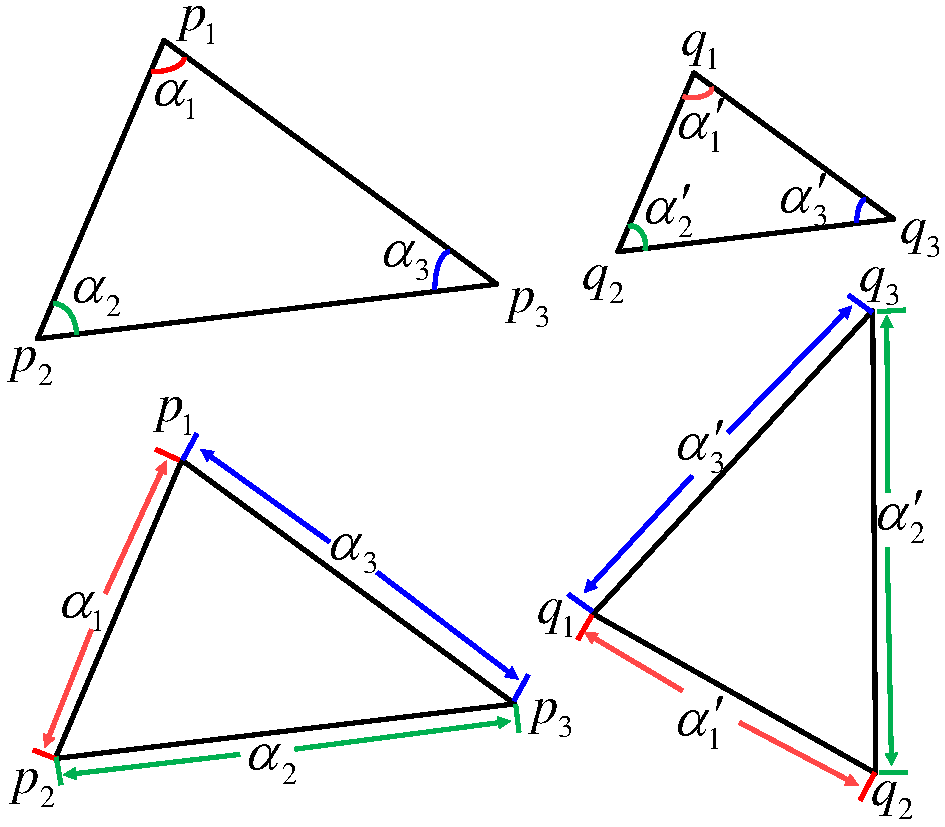
\includegraphics[width=0.8\linewidth]{figures/diagram.jpg}
  \caption{Third-order potential schematic diagram. The geometric constraints: internal angle invariance in 2D (up), and edge length invariance in 3D case (bottom).}
\label{fig:TO}
\end{figure}

%-------------------------------------------------------------------------
\subsection{Sampling strategy}
\label{subsec:sampling}

Algorithm~\ref{alg2} depends on all potential elements. 
We next discuss the issue of how to sample the feature tuples to build potential items, which determines the size $|\theta_N|$ and influences matching accuracy.

Given two feature sets $P_1$ and $P_2$ with $N_1$ and $N_2$ features respectively,
a potential element may be obtained by using two feature tuples sampled from each feature set separately.
For $N$th-order matching, a naive way to construct the potential elements is as follows:
first find all feature tuples for $P_1$ and $P_2$, as $F_1$ and $F_2$; then $\forall (f_{i_1}^1, f_{i_2}^1, \cdots, f_{i_N}^1)\in F_1$,
calculating the potentials for $(f_{i_1}^1, f_{i_2}^1, \cdots, f_{i_N}^1)$ with all feature tuples in $F_2$.
This naive method is very expensive, which is why sampling is used.
Different sampling strategies can be chosen for different applications,
we employ random sampling for general feature matching problems. 
%as there is no guidance to provide a better sampling method.

Our sampling works as following: randomly sampling $t_1$ feature tuples for $P_1$, and full sampling for $P_2$ (to find all $N_2^N$ feature tuples).
For $P_1$, in order to cover all features in $P_1$ in $F_1$, we repeatedly take one feature as a required element,
and then  randomly choose $t_1$ feature tuples containing these required element.
We repeat this process until all features in $P_1$ have been chosen once as a required element.
Then, $\forall (f_{i_1}^1, f_{i_2}^1, \cdots, f_{i_N}^1)\in F_1$, we find the $k$ most similar features in $F_2$ to build $k$ potential elements as $\phi_i^k$.
Combining all the potential elements obtained, we form the desired potential element set $\theta_N = \{\phi_i^k\}_{i=1}^{N_1 t_1}$, with the size $|\theta_N| = N_1 t_1 k$.
The parameters $t_1$ and $k$ must be chosen according to the size of the feature sets. 
For $P_1$, the sampling cost is $O(N_1\, t_1\,  k\log N_1)$.
In practice, for two feature sets each with hundreds points, 
we take $t_1 \approx 50$ and $k \approx 300$ for third-order and higher-order (e.g. fourth-order) matching.
The experiments demonstrate that this sampling approach works well.


The most important part of the sampling is to use the supersymmetry of the affinity tensor.
An $N^{th}$-order supersymmetric affinity tensor must satisfy:
\begin{eqnarray}
\label{equ:noredun}
\forall (i_1,i_2,\cdots,i_N),(j_1,j_2,\ldots,j_N) \in \theta_N,\nonumber\\(i_1,i_2,\cdots,i_N)\neq\Omega(j_1,j_2,\cdots,j_N)
\end{eqnarray}
where $\Omega$ is an arbitrary permutation.
Thus, we use a sampling constraint that the sets of feature tuples $F_1$ obtained from the sampling process, should have no repetition, in the sense that
\begin{eqnarray}
\label{equ:noredun2}
\forall (f_{i_1}^1,f_{i_2}^1,\cdots,f_{i_N}^1),(f_{j_1}^1,f_{j_2}^1,\cdots,f_{j_N}^1) \in F_1,\nonumber\\ (f_{i_1}^1,f_{i_2}^1,\cdots,f_{i_N}^1)\neq\Omega(f_{j_1}^1,f_{j_2}^1,\cdots,f_{j_N}^1)
\end{eqnarray}
and $\Omega$ is arbitrary permutation.
This sampling constraint eliminates overlaps that may appear in the potential elements $\theta_N$.

Earlier work~\cite{Duchenne_etal09,Zass08} ever adopted random sampling, 
but failed to impose any constraint on the sampling process,
leading to the possibility that feature tuples may include repetition.
For example, for third-order matching, it is possible that a feature tuple $(f_{i_1}^1, f_{i_2}^1, f_{i_3}^1)$ may be sampled from $P_1$ and $(f_{i_1}^2, f_{i_2}^2, f_{i_3}^2)$ from $P_2$, and also a feature tuple $(f_{i_1}^1, f_{i_3}^1, f_{i_2}^1)$ sampled from $P_1$ and $(f_{i_1}^2, f_{i_3}^2, f_{i_2}^2)$ from $P_2$. That will create two tensor elements $\phi_3(s_{i_1}, s_{i_2}, s_{i_3})$ with index $(s_{i_1}, s_{i_2}, s_{i_3})$ and $\phi_3(s_{i_1}, s_{i_3}, s_{i_2})$ with index $(s_{i_1}, s_{i_3}, s_{i_2})$, which are the same. However, we just need one tensor element to express the affinity measure on the assignment group $(s_{i_1}, s_{i_2}, s_{i_3})$. 
This repetitive problem not only makes the potential elements redundant but also affects the accuracy of the power iteration, 
because the numbers of each tensor element may not be equal and some elements may be used more than once during the iteration progress.
Therefore, our sampling method reduces the sampling cost, while also improving the accuracy of the power iteration.
